\documentclass[11pt]{article}
\usepackage[english]{babel}
\usepackage{minted}
\usepackage{amsmath}
\usepackage{amsthm}
\usepackage{graphicx}
\usepackage{subcaption}
\usepackage{multirow}
\usepackage{booktabs}
\usepackage[left=25mm, top=25mm, bottom=30mm, right=25mm]{geometry}
\usepackage[colorlinks=true, linkcolor=blue, urlcolor=cyan]{hyperref}

\title{COL334 Assignment 3}
\author{Sayam Sethi}
\date{October 2021}

\begin{document}

\maketitle

\tableofcontents

\section{Part 1}

\subsection{Plots}
\begin{figure}[H]
  \begin{subfigure}{0.5\textwidth}
    \centering
    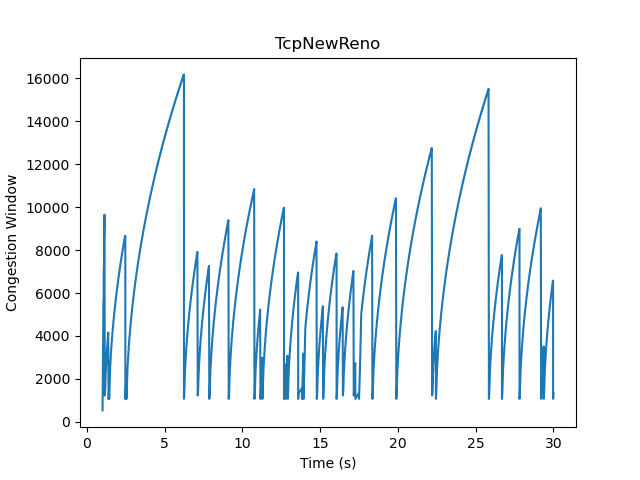
\includegraphics[width=0.9\linewidth]{Q1/outputs/TcpNewReno.png}
    \caption{TcpNewReno}
  \end{subfigure}
  \begin{subfigure}{0.5\textwidth}
    \centering
    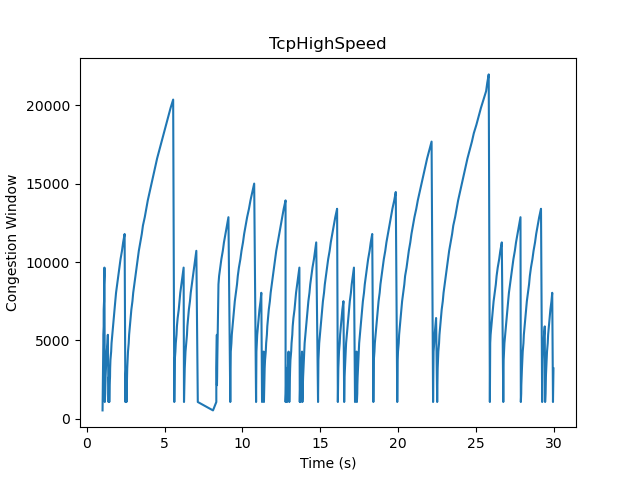
\includegraphics[width=0.9\linewidth]{Q1/outputs/TcpHighSpeed.png}
    \caption{TcpHighSpeed}
  \end{subfigure}
\end{figure}

\begin{figure}[H]
  \begin{subfigure}{0.5\textwidth}
    \centering
    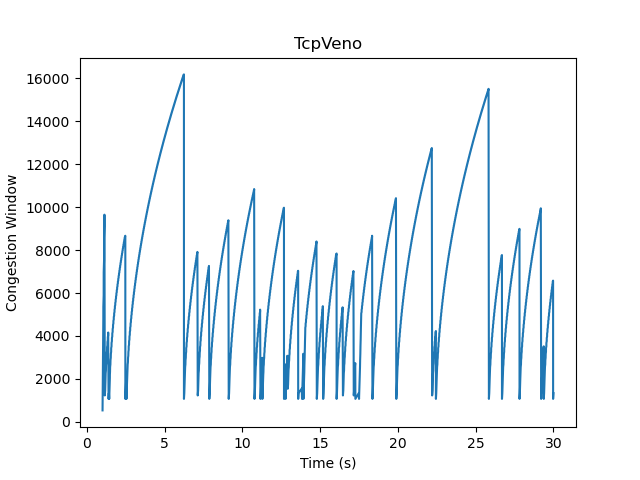
\includegraphics[width=0.9\linewidth]{Q1/outputs/TcpVeno.png}
    \caption{TcpVeno}
  \end{subfigure}
  \begin{subfigure}{0.5\textwidth}
    \centering
    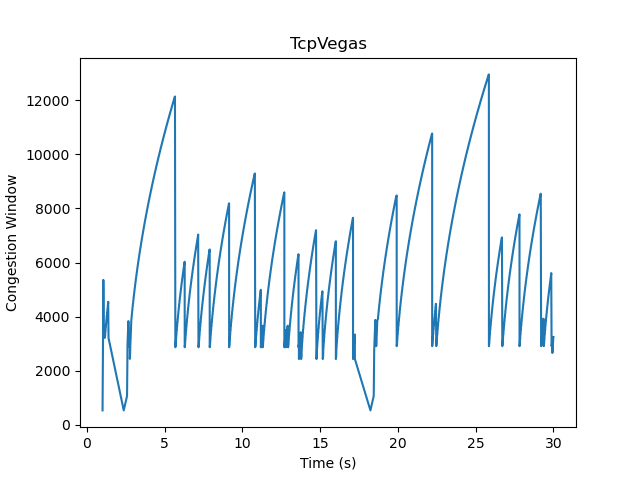
\includegraphics[width=0.9\linewidth]{Q1/outputs/TcpVegas.png}
    \caption{TcpVegas}
  \end{subfigure}
\end{figure}

\subsection{Dropped Packets}
\begin{enumerate}
  \item \textbf{TcpNewReno:} There are $38$ dropped packets
  \item \textbf{TcpHighSpeed:} This also has $38$ dropped packets
  \item \textbf{TcpVeno:} This also has $38$ dropped packets
  \item \textbf{TcpVegas:} This has $39$ dropped packets
\end{enumerate}

\subsection{Observations}

\subsubsection{TcpNewReno}
\begin{itemize}
    \item There is linear increase in the congestion window in the slow start phase.
    \item This changes to slow increase in the congestion avoidance phase, which leads to lesser chances of packet drop.
    \item The slow start threshold is halved with each drop which leads to the decrease in the maximum congestion window after each drop until it start increasing again after it becomes small.
\end{itemize}

\subsubsection{TcpHighSpeed}
\begin{itemize}
  \item This protocol does not visibly have any slow start phase, which leads to the large increase in the congestion window initially and that stabilises once the congestion window is relatively higher.
  \item In the case of packet drop, the congestion window decreases as a function of the congestion window. Therefore, there is lesser decrease in the congestion window in case of packet drop when the congestion window is smaller.
  \item Therefore, this model will be suitable for links which have high data link capacity since it handles packet drops efficiently when the congestion window is larger.
\end{itemize}

\subsubsection{TcpVeno}
\begin{itemize}
  \item The plot is exactly the same as the plot of \texttt{TcpNewReno}.
  \item On examining the implementation of \texttt{TcpVeno} further, we notice that the implementation calls corresponding functions of \texttt{TcpNewReno} with a difference being in the handling of packet drop.
  \item The different implementation in handling drops is not visible for the duration of the simulation, therefore we can conclude that \texttt{TcpVeno} is almost the same as \texttt{TcpNewReno} in practical scenarios for small connection durations.
\end{itemize}

\subsubsection{TcpVegas}
\begin{itemize}
  \item This protocol works on the basis of delay instead of the packet drops.
  \item Therefore, the model is \textit{conservative} in increasing the congestion window and when the delay increases, it avoids it by decreasing the congestion window.
\end{itemize}


\section{Part 2}

\subsection{Varying Channel Rates}
\subsubsection{Observation}
From the plots given in Section~\ref{sec:channel}, we notice that the amount of variation in the congestion window per second increases. This is because it becomes possible to transmit more number of packets over the link. The only limitation is the \textit{application rate} which is set at 2Mbps. This is also consistent with the last three graphs being almost identical. Additionally, we state that the large variation in congestion window for larger channel rates is because of larger frequency of packet drops. This happens since even though the error model is unchanged, the number of packets being transmitted each second increases.

\subsubsection{Plots}\label{sec:channel}
\begin{figure}[H]
  \centering
  \begin{tabular}[c]{cc}
    \begin{subfigure}[c]{0.5\textwidth}
      \centering
      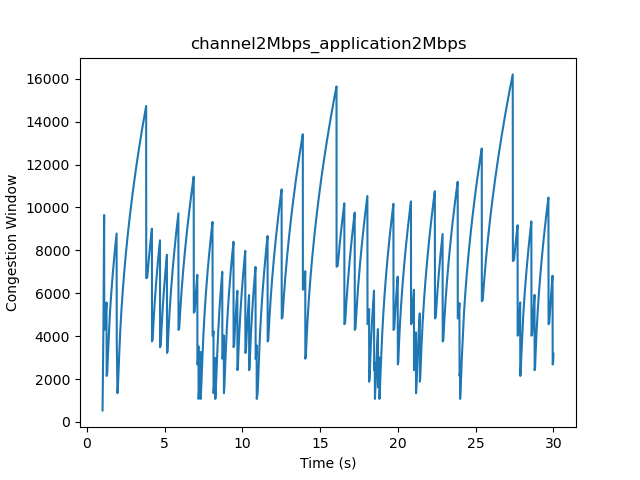
\includegraphics[width=\textwidth]{Q2/outputs/channel2Mbps_application2Mbps.png}
      \caption{Link rate = 2Mbps}
    \end{subfigure}&

    \begin{subfigure}[c]{0.5\textwidth}
      \centering
      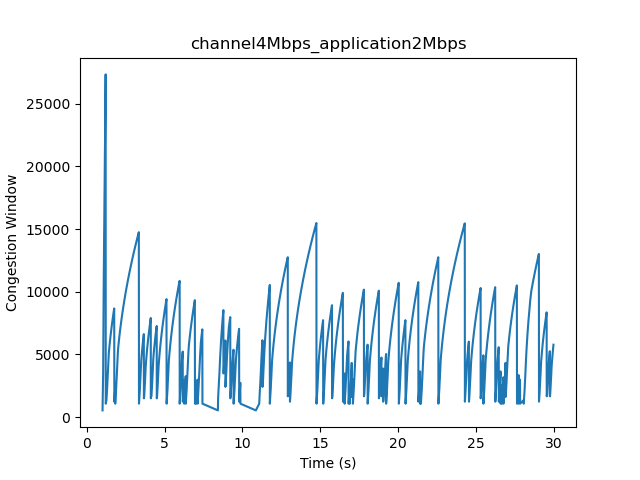
\includegraphics[width=\textwidth]{Q2/outputs/channel4Mbps_application2Mbps.png}
      \caption{Link rate = 4Mbps}
    \end{subfigure}\\

    \begin{subfigure}[c]{0.5\textwidth}
      \centering
      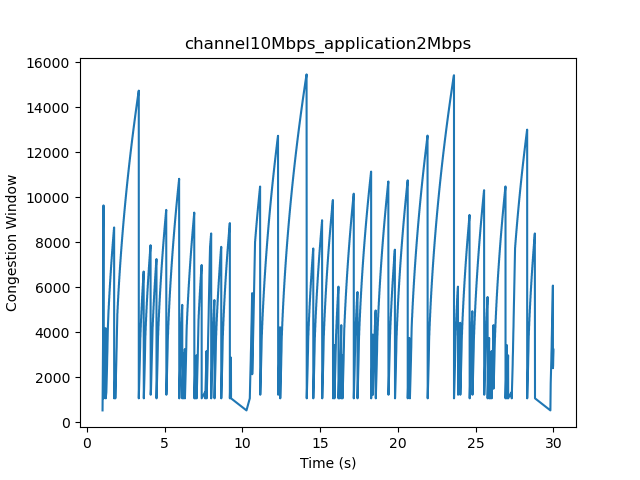
\includegraphics[width=\textwidth]{Q2/outputs/channel10Mbps_application2Mbps.png}
      \caption{Link rate = 10Mbps}
    \end{subfigure}&

    \begin{subfigure}[c]{0.5\textwidth}
      \centering
      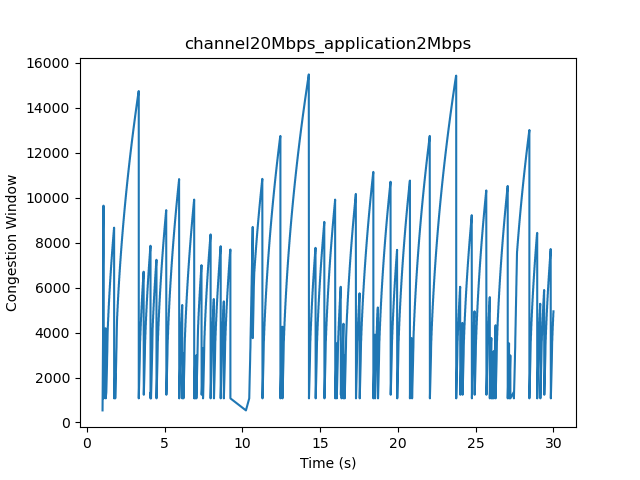
\includegraphics[width=\textwidth]{Q2/outputs/channel20Mbps_application2Mbps.png}
      \caption{Link rate = 20Mbps}
    \end{subfigure}\\

    \multicolumn{2}{c}
      {\begin{subfigure}[c]{0.5\textwidth}
        \centering
        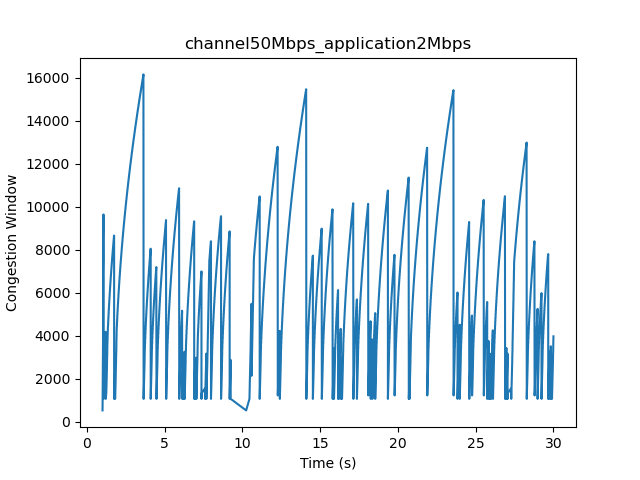
\includegraphics[width=\textwidth]{Q2/outputs/channel50Mbps_application2Mbps.png}
        \caption{Link rate = 50Mbps}
      \end{subfigure}}
    
  \end{tabular}
\end{figure}

\subsection{Varying Application Rates}
\subsubsection{Observation}
From the plots in Section~\ref{sec:application}, we observe that for smaller application rates, the congestion avoidance phase stays for a longer time. However, as the application rate increases, the shift happens towards the slow start phase. From this, we infer that the drop rate increases for larger application rates. The source of congestion in this case becomes the link as the application rate rises. For the largest application rate, there is a region of considerably low congestion window. This implies that the application has to slow down its functioning to accomodate the congestion in the network.

\subsubsection{Plots}\label{sec:application}
\begin{figure}[H]
  \centering
  \begin{tabular}[c]{cc}
    \begin{subfigure}[c]{0.5\textwidth}
      \centering
      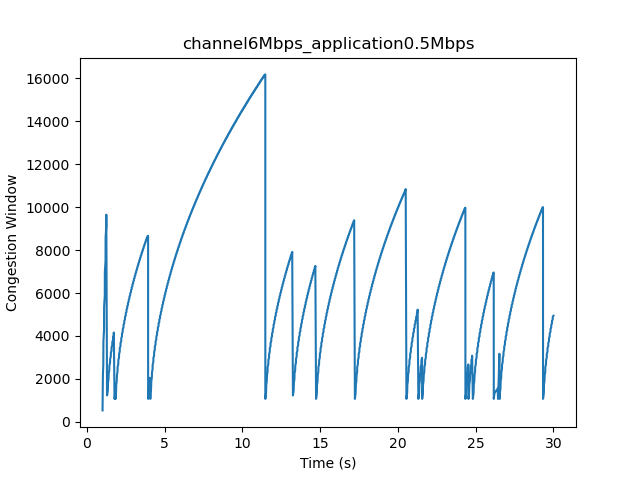
\includegraphics[width=\textwidth]{Q2/outputs/channel6Mbps_application0.5Mbps.png}
      \caption{Link rate = 2Mbps}
    \end{subfigure}&

    \begin{subfigure}[c]{0.5\textwidth}
      \centering
      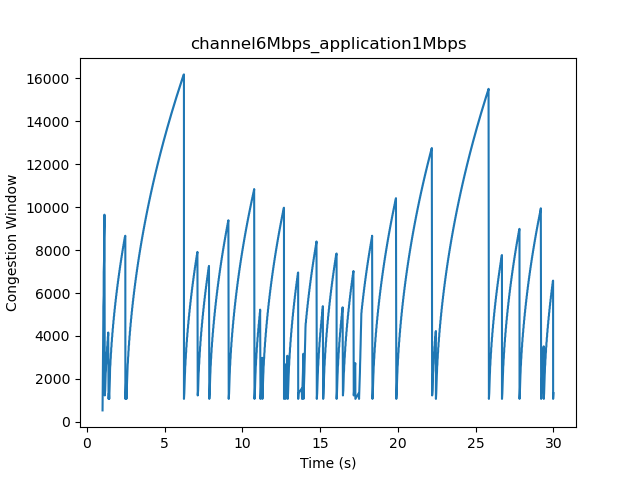
\includegraphics[width=\textwidth]{Q2/outputs/channel6Mbps_application1Mbps.png}
      \caption{Link rate = 4Mbps}
    \end{subfigure}\\

    \begin{subfigure}[c]{0.5\textwidth}
      \centering
      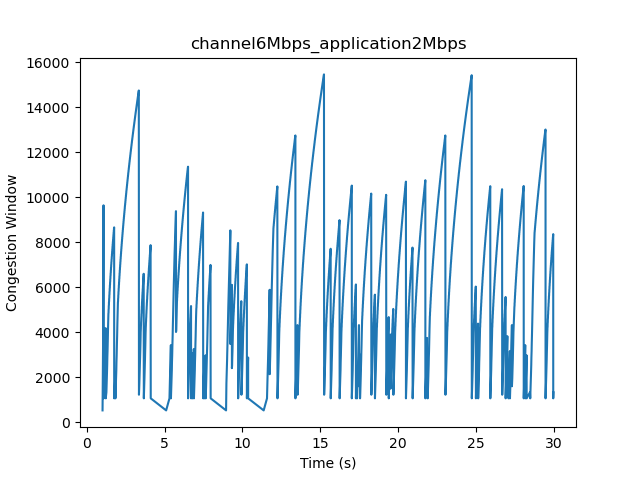
\includegraphics[width=\textwidth]{Q2/outputs/channel6Mbps_application2Mbps.png}
      \caption{Link rate = 10Mbps}
    \end{subfigure}&

    \begin{subfigure}[c]{0.5\textwidth}
      \centering
      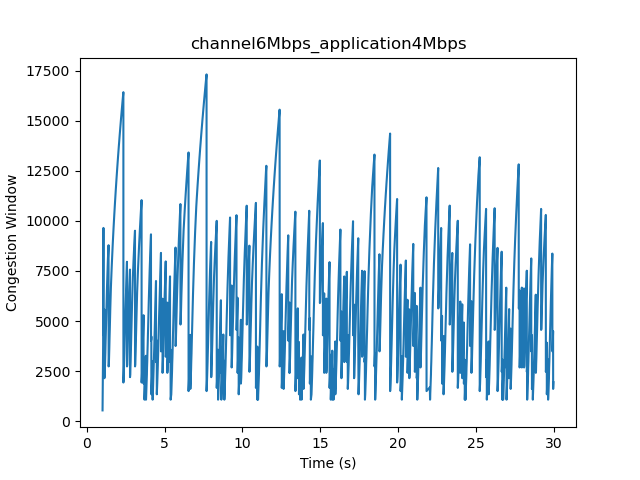
\includegraphics[width=\textwidth]{Q2/outputs/channel6Mbps_application4Mbps.png}
      \caption{Link rate = 20Mbps}
    \end{subfigure}\\

    \multicolumn{2}{c}
      {\begin{subfigure}[c]{0.5\textwidth}
        \centering
        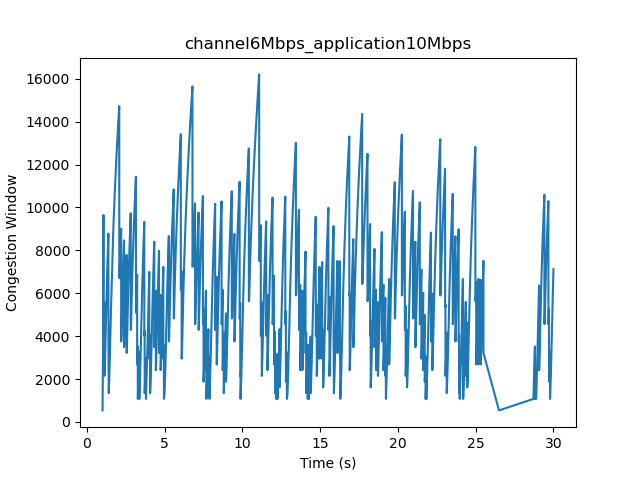
\includegraphics[width=\textwidth]{Q2/outputs/channel6Mbps_application10Mbps.png}
        \caption{Link rate = 50Mbps}
      \end{subfigure}}
    
  \end{tabular}
\end{figure}

\section{Part 3}

\subsection{Configuration 1}
There are $113$ dropped packets.
\begin{figure}[H]
  \centering
  \begin{tabular}[c]{cc}
    \begin{subfigure}[c]{0.5\textwidth}
      \centering
      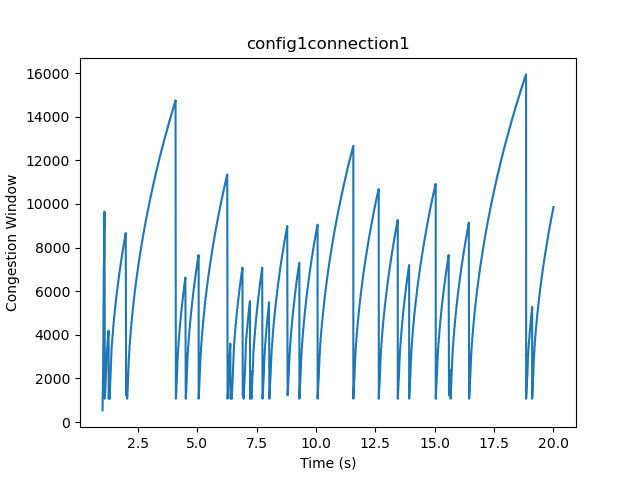
\includegraphics[width=\textwidth]{Q3/outputs/config1connection1.png}
      \caption{Connection 1}
    \end{subfigure}&

    \begin{subfigure}[c]{0.5\textwidth}
      \centering
      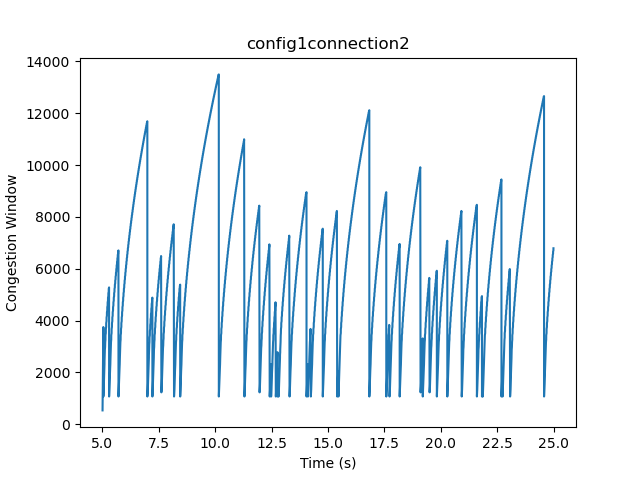
\includegraphics[width=\textwidth]{Q3/outputs/config1connection2.png}
      \caption{Connection 2}
    \end{subfigure}\\

    \multicolumn{2}{c}
      {\begin{subfigure}[c]{0.5\textwidth}
        \centering
        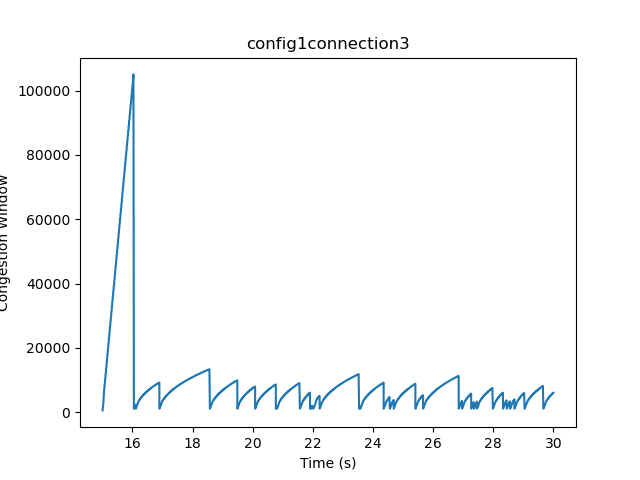
\includegraphics[width=\textwidth]{Q3/outputs/config1connection3.png}
        \caption{Connection 3}
      \end{subfigure}}
  \end{tabular}
\end{figure}

\subsection{Configuration 2}
There are $112$ dropped packets in this case.
\begin{figure}[H]
  \centering
  \begin{tabular}[c]{cc}
    \begin{subfigure}[c]{0.5\textwidth}
      \centering
      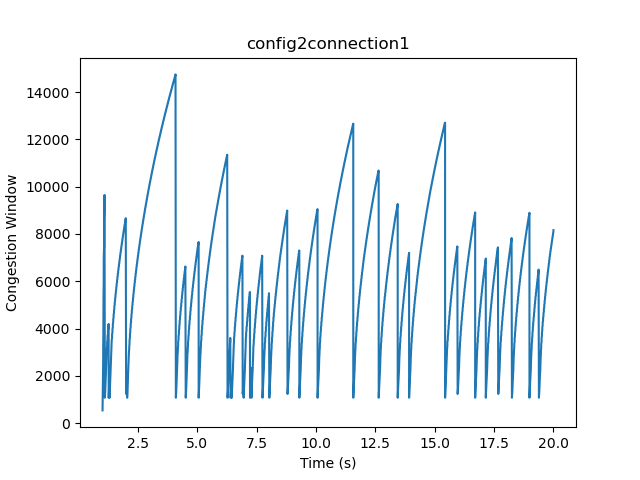
\includegraphics[width=\textwidth]{Q3/outputs/config2connection1.png}
      \caption{Connection 1}
    \end{subfigure}&

    \begin{subfigure}[c]{0.5\textwidth}
      \centering
      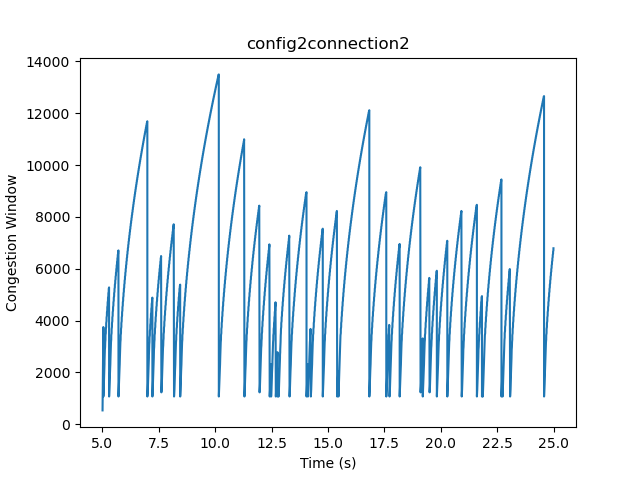
\includegraphics[width=\textwidth]{Q3/outputs/config2connection2.png}
      \caption{Connection 2}
    \end{subfigure}\\

    \multicolumn{2}{c}
      {\begin{subfigure}[c]{0.5\textwidth}
        \centering
        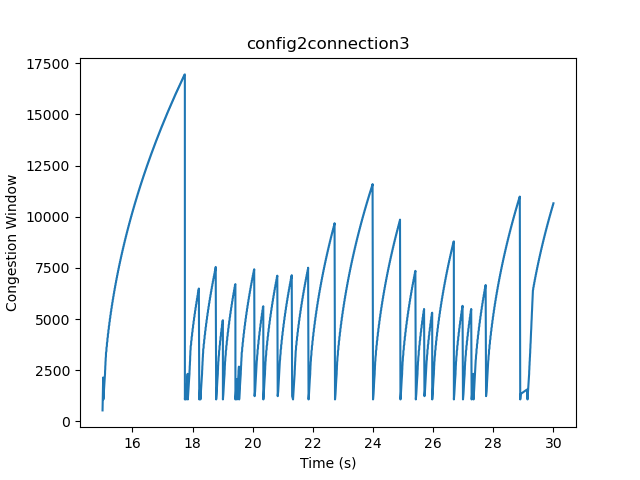
\includegraphics[width=\textwidth]{Q3/outputs/config2connection3.png}
        \caption{Connection 3}
      \end{subfigure}}
  \end{tabular}
\end{figure}

\subsection{Configuration 3}
There are $110$ dropped packets.
\begin{figure}[H]
  \centering
  \begin{tabular}[c]{cc}
    \begin{subfigure}[c]{0.5\textwidth}
      \centering
      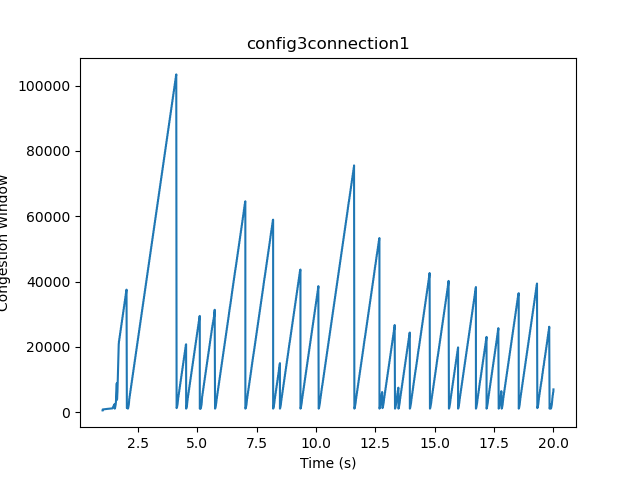
\includegraphics[width=\textwidth]{Q3/outputs/config3connection1.png}
      \caption{Connection 1}
    \end{subfigure}&

    \begin{subfigure}[c]{0.5\textwidth}
      \centering
      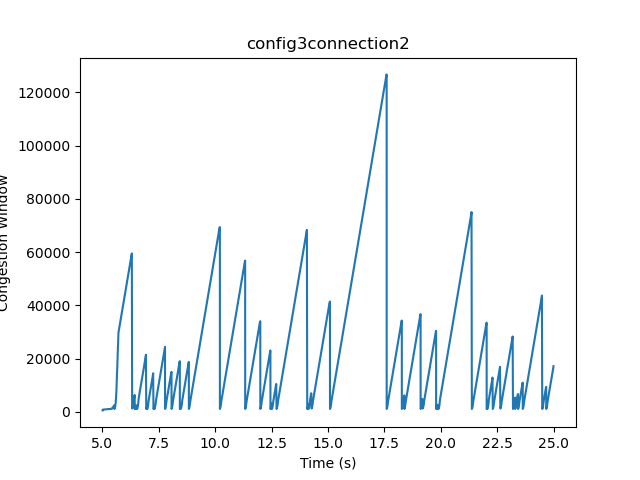
\includegraphics[width=\textwidth]{Q3/outputs/config3connection2.png}
      \caption{Connection 2}
    \end{subfigure}\\

    \multicolumn{2}{c}
      {\begin{subfigure}[c]{0.5\textwidth}
        \centering
        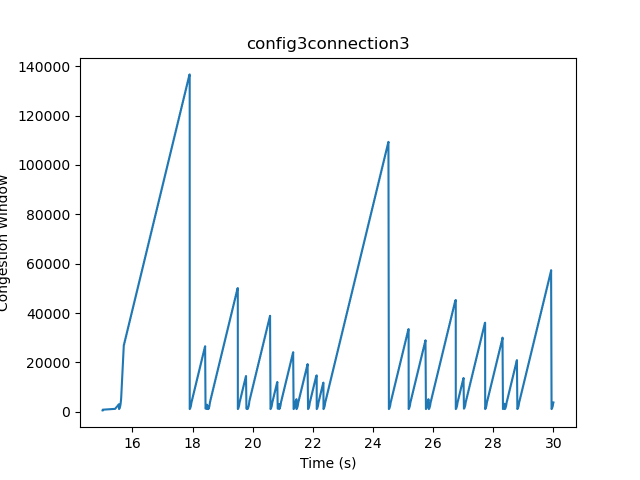
\includegraphics[width=\textwidth]{Q3/outputs/config3connection3.png}
        \caption{Connection 3}
      \end{subfigure}}
  \end{tabular}
\end{figure}

\subsection{Observations}
\textit{Note:} Two error models (with the same paramters) have been used, one for each link
\begin{enumerate}
    \item The plots for connection $1, 2$ is the same for configurations $1$ and $2$ since the error models and links are independent.
    \item Looking at the plots, we notice that the average congestion window size is higher whenever we use \texttt{TcpNewRenoCSE} instead of \texttt{TcpNewReno} for a single connection
    \item Also, considering connection $1, 2$ for configurations $1$ and $3$, we notice that congestion window size reached much higher values in configuration $3$ as compared to configuration $2$.
    \item Because of large number of packet drops on the first link, for both models, both the slow start as well as congestion avoidance states are achieved.
    \item In the case of configuration $3$, for connection $3$, the slow start phase increases the congestion window slightly and then it shifts to congestion avoidance, thus the large linear increase.
    \item However, in the case of configuration $1$, for connection $3$, the protocol largely remains in slow start phase which leads to relatively lower congestion window sizes.
\end{enumerate}


\section{Code Explanation}
The code for all parts has been modified from \texttt{examples/tutorial/sixth.cc} provided in the \texttt{ns3} tutorial. Command line arguments have been taken and a shell script has been written for each part. To run the code, each folder needs to be copied to the \texttt{scratch} directory of the \texttt{ns3} folder after which entering the directory of corresponding part and running the shell script suffices. The plots have been made using \texttt{plot.py} file present in the root submission directory.

\end{document}
